\chapter{Artificial Intelligence Agents}
\label{AIAgents}

My implementation of Durak features five distinct agents: Random, Greedy, Smart, Minimax, and Monte Carlo Tree Search. In this chapter, we will delve into the characteristics and behaviors of each of these agents in order to gain a better understanding of their nature. 

\section{Random Agent}
The random agent simply selects an action at random, as its name suggests. It serves as a foundational reference point for comparison with more advanced algorithms. 

\begin{figure}[h]
\captionsetup{justification=centering}
\begin{lstlisting}
function Move(gameView: GameView)
    cards = gameView.Actions(excludePassTake: true)

    // cannot attack/defend
    if cards.Count == 1 and cards[0] is null
        return null
    
    // include the case when the ai can decide to pass/take
    // even if it can defend/attack (20% chance)
    // allow only when the first attack was given
    rn = random number between 0 and 100
    if rn <= 20 and gameView.bout.GetAttackingCards().Count > 0
        return null
    
    return a random card from cards
\end{lstlisting}
\caption{Pseudocode of Move method of the Random agent}
\label{fig:randomMove}
\end{figure}

Figure 4.1 presents the Move method for the Random agent. When there are no available moves to be made (i.e., the \texttt{gameView.Actions(...)} method returns an null at the first index of the list), the agent interprets this as a Pass if it is the attacker, or as a Take if it is the defender. Given that there are multiple options available, the random agent has a 20\% probability of randomly deciding to either Pass or Take the card, depending on its role. There may actually be no good reason to have a fixed probability of passing on each move, but I implemented this policy early on and did not want to disrupt experiments by changing it later.


\section{Rule-Based Heuristic Agents}

Rule-based heuristic agents are agents that use a set of predefined rules, heuristics or strategies to make decisions \citep{millington_funge_2009}. These rules are designed to capture the key characteristics of a problem or task, and they are used by the agent to determine the best course of action to take in a given situation.

The strategies employed by the agents in this section were developed through the accumulation of experience gained over multiple games. These strategies are not guaranteed to produce victory in every game, but they increase the chances of winning by making moves based on predefined rules. 

\subsection{Greedy Agent}

I have observed through years of playing this game that the best move in any given game state is often to play the card with the lowest value. This approach is advantageous because it allows the player to save strong cards for later in the game, increasing the chances of winning. Conversely, using high value cards for attack and defense in the early game and reserving weak cards for later can lead to a loss. Additionally, playing the lowest value cards allows the player to draw stronger cards from the deck, thereby building a stronger hand over the course of the game. As such, the greedy agent employs a predetermined strategy in which it selects the lowest ranked card for attack or defense based on the current turn. Specifically, if the agent is attacking, it will choose the lowest valued card to attack with. If the agent is defending, it will select the lowest valued card that can defend against an incoming attack. To provide an example, consider the scenario described in section \ref{illustration}, in which Player A attacks with 6$\textcolor{red}{\heartsuit}$ as a first turn. Among all the possible options, which includes 8$\textcolor{red}{\heartsuit}$, A$\textcolor{red}{\heartsuit}$, 6$\textcolor{black}{\spadesuit}$, to select to defend against the attacking card, Player B chooses 8$\textcolor{red}{\heartsuit}$ which is the lowest rank value in their hand to defend against the attacking card. The 6$\textcolor{black}{\spadesuit}$ card was not selected because it is a trump card and therefore has a higher value than non-trump cards, thus, it has higher value than 8$\textcolor{red}{\heartsuit}$. This decision-making process aligns with the strategy employed by a greedy agent, which aims to maximize their own short-term gain at the expense of potentially more optimal long-term outcomes \citep{AI4Ed}.

\begin{figure}[h]
\captionsetup{justification=centering}
\begin{lstlisting}
function Move(gameView)
    moves = PossibleMoves(gameView)
    if HasNull(moves) is true
        return NULL
    else
        return GetCard(moves, gameView)

function GetCard(possibleCards, gView)
    noTrumpCards = SelectNonTrumpCards(possibleCards)
    if size of noTrumpCards is 0
        if EarlyGame(gView) is true
            if size of BoutACards(gView) > 0 and Turn(gView) == ATTACK
                return NULL
            else
                return LowestRank(possibleCards)
        else
            return LowestRank(possibleCards)
    else
        return LowestRank(noTrumpCards)
\end{lstlisting}
\caption{Pseudocode of the Move method}
\label{fig:greedyMove}
\end{figure}

The pseudocode shown in Figure \ref{fig:greedyMove} outlines the steps taken by the greedy agent to evaluate its options and make a decision. Specifically inside the \texttt{Move} method, the agent utilizes the \texttt{PossibleMoves} method to obtain a list of all possible actions it can take based on the current game state. \texttt{HasNull(moves)} detects if no actions are available. If that's the case, the agent will either pass or take a card, depending on its role in the game. However, if there are available actions, the agent will use the \texttt{GetCard} method to identify the card with the lowest value among the possible moves and select it as its next action. To ensure that the greedy agent is able to maximize its gain, we select the non-trump cards from the list of available options when determining the agent's next move. If the agent has a choice between non-trump cards, it will naturally select the one with the lowest rank value. However, if the agent only has trump cards to choose from, we must consider the \textbf{stage} of the game: early or end game. If the greedy agent is acting as an attacker and has the option to pass the attack, it is generally better to do so during the early game, as this allows the agent to preserve its trump cards for use in the end game, when they are likely to be more valuable. On the other hand, if the greedy agent is defending, it does not matter whether it uses trump cards or not at any stage of the game, as giving up these cards is preferable to taking the entire bout.

\subsection{Smart Agent}
\label{smart}
A smart agent using rule-based heuristics can exhibit improved performance compared to a greedy agent. This is because the smart agent utilizes rules that take into account the opponent's hand, providing a strategic advantage. One specific rule that may be implemented during the defensive stage is the selection of a defending card with a rank that the opponent does not possess. If it is not possible to utilize the aforementioned defensive strategy due to the opponent holding cards of the same rank as the available defending cards, the agent may choose to defend with the card of the lowest rank.  The implementation of the method is represented in Figure \ref{fig:defStratSmart}. This rule aims to prevent further attacks in the same bout by mitigating the opponent's options. While this rule may not be the most effective in every scenario, it has demonstrated successful outcomes in certain situations.

\begin{figure}[h]
\captionsetup{justification=centering}
\begin{lstlisting}
Card? DefendingStrategy(List<Card> oHand, List<Card> cards)
    for each card(*@$\in$@*)cards do
        if (oHand) contains any cards with the same rank as (card) then
            return (card)
    return GetLowestRank(cards);
\end{lstlisting}
\caption{Pseudocode of the \texttt{Move} method of the Greedy agent, where \texttt{oHand} is a list of cards in the opponent's hand and \texttt{cards} is a list of possible cards to defend with}
\label{fig:defStratSmart}
\end{figure}

Moreover, a smart agent may employ a strategy that leverages the concept of \textbf{weaknesses} discussed in Section \ref{weaknessConcept} in order to gain an advantage. \textit{If player P only possesses a single weakness at rank r during their turn, then they have a winning strategy} \citep{Bonnet2016TheCO}. In the example presented in Section \ref{weaknessConcept}, player P possesses a weakness of rank 10. According to the aforementioned statement, this implies that player P has a winning strategy and can outmaneuver their opponent. This is indeed the case. To initiate the attack, player P can utilize all non-weakness rank cards, such as the K$\textcolor{red}{\diamondsuit}$. The opponent must take the attacking card, as they are unable to defend against it due to K being a non-weakness rank. With the new bout, it is player P's turn to initiate an attack. They choose to attack with the 10$\textcolor{red}{\heartsuit}$, which has a weakness rank. In response, player O defends with the Q$\textcolor{red}{\heartsuit}$. The turn then returns to player P, who attacks with their final card, the 10$\textcolor{black}{\spadesuit}$, which also has a weakness rank. Although player O is able to defend against this attack, they become the loser because they are the only player remaining with cards.

One limitation of this strategy is that it is only applicable in open-world environments, where the player is able to gather information about their opponent's hand in order to identify weakness in their hand.  Nonetheless, the weakness strategy can still be utilized in closed-world games, but only in the endgame when the deck is exhausted. This is because when players have used up the entire deck, it implies that certain cards played during the bout have been placed in the discard pile. This allows the players to deduce the opponent's cards and successfully use the strategy for their advantage. A smart agent adheres to this principle, which, while not being a common occurrence in the game, is highly effective and ensures victory for the smart agent.

\section{Minimax Agent}
\label{minimax}

In this section, we will discuss an agent that uses the minimax algorithm to play Durak. Specifically, we will examine the importance of the parameters in the minimax algorithm and the heuristic functions included in the Durak Command Line Interface (CLI) for evaluating the game state.

The minimax algorithm is a decision-making algorithm often used in two-player turn-based perfect information games, such as chess, tic-tac-toe, and Go \citep{AI4Ed}. It is called minimax because it tries to minimize the maximum loss that a player can incur. It operates by using the recursion to explore a game tree, with each node representing a potential game state, and the branches representing the possible moves that can be made from that state. The minimax algorithm then traverses the game tree, evaluating the value of each node recursively. When applied to the entire tree, the minimax values produced by this algorithm accurately reflect the outcome of the game with perfect play by both players. The pseudocode of the minimax algorithm is illustrated in Figure \ref{fig:minimaxPseudocode}. To explore the potential game states, the minimax algorithm creates the copy, \texttt{game.Copy()}, of the state to ensure that the original game state cannot be changed after making possible moves. It is important to note that the following discussion of the algorithm assumes an open Durak environment, in which all players have access to the visible cards. This allows the game state to be freely cloned without letting the agent to see the hidden information. Section \ref{closedWorld} will address the algorithm's handling of the closed world environment, in which there is hidden information.

\begin{figure}[h]
\captionsetup{justification=centering}
\begin{lstlisting}
function minimax(game, depth, out bestMove)
    if depth = MAX_DEPTH or game is in terminal state
        return the heuristic value of state
        
    bestVal = game.turn == 1 ? -infinity : +infinity
        
    for each card of game.PossibleMoves()
        stateCopy = game.Copy()
        stateCopy.Move(card)
        v = minimax(stateCopy, depth + 1, _)
		
        if game.turn == 1 && v > bestVal or game.turn == 2 && v < bestVal then
            bestVal = v;
            bestMove = card;
			
    return bestVal
\end{lstlisting}
\caption{Pseudocode for the minimax algorithm}
\label{fig:minimaxPseudocode}
\end{figure}

Due to the exponential increase in the size of the tree as the search depth increases, it is often infeasible to search the entire tree. As a result, the minimax algorithm must be terminated at some depth (\texttt{MAX\_DEPTH}), and the minimax value for a given node is approximated using a heuristic evaluation function. The heuristic function assigns a score to the current game state based on a set of predefined criteria, which will be discussed further in this section. While the use of a heuristic evaluation function introduces some error into the minimax values, it allows the algorithm to produce reasonable results in a reasonable amount of time.

\subsection{Basic Heuristic}
The basic heuristic function utilizes predetermined criteria to evaluate the game state, using the contents of the players' hands, the size of the players' hands, and the presence of any weaknesses. It should be noted that this is not the only method of evaluating the state, and there are potentially numerous other criteria that could be incorporated into the heuristic function. However, the criteria mentioned are considered to be the primary ones used in the basic heuristic function.

\begin{figure}[h]
\captionsetup{justification=centering}
\begin{lstlisting}
function ConvertHandToValue(hand: List of Card, gw: GameView)
    TOTALCARDS = 9
    value = 0

    for each card in hand
        if gw.includeTrumps is true and card.suit == gw.trumpCard.suit
            value = value + card.rank + TOTALCARDS
        else
            value = value + card.rank

    return value

function EvaluatePlayerHandToValue(gw: GameView)
    return ConvertHandToValue(gw.players[0].GetHand(), gw) - 	ConvertHandToValue(gw.players[1].GetHand(), gw)
\end{lstlisting}
\caption{Pseudocode of partial basic heuristic function evaluating the state based on the players' hand value}
\label{fig:BHPlayersHandValue}
\end{figure}

In order to evaluate the state of a card game based on the cards held by each player, the heuristic function begins by computing the individual hand value of each player. Prior to beginning this calculation, the value of each card must be determined. This can be done by assigning the value of a card as its rank. For example, if player P holds the cards 6$\textcolor{red}{\heartsuit}$ and A$\textcolor{red}{\heartsuit}$, the value of their hand would be 20 (6 + 14). Trump cards are powerful, so we assign them a higher value. To achieve this, we calculate the value of a trump card by adding its rank to the total number of ranks in the deck. For example, the value of a trump card with rank 6 would be calculated as 6 + the total number of ranks in the deck (6, 7, ..., K, A). After the individual hand value of each player has been calculated, a basic heuristic function may be used to evaluate the game state. This can be done by subtracting the hand value of player P from that of player O. The result of this calculation can then be used to represent the game state. How this is achieved can be viewed in Figure \ref{fig:BHPlayersHandValue}. It should be noted that this method of evaluating the game state is only suitable for use when the players have an equal number of cards. In past experiments, using this evaluation method with players who have an equal number of cards has been found to produce more accurate and reliable results.

\begin{figure}[h]
\captionsetup{justification=centering}
\begin{lstlisting}
function EvaluateHandSize(gw: GameView)
    pHandSize = gw.players[0].GetNumberOfCards()
    oHandSize = gw.players[1].GetNumberOfCards()

    if gw.isEarlyGame is true
        pHandSize = pHandSize
    else
        pHandSize = pHandSize * 15
    if gw.isEarlyGame is true
        oHandSize = oHandSize
    else
        oHandSize = oHandSize * 15

    return (pHandSize - oHandSize) * -1
\end{lstlisting}
\caption{Pseudocode of partial basic heuristic function evaluating the state based on the players' hand size value}
\label{fig:BHPlayerHandSize}
\end{figure}

Another criterion that may be used to evaluate the state of a card game is the size of the players' hands. The number of cards held by each player can provide insight into the likely outcome of the game. This can be done by subtracting the size of player P's hand from that of player O's hand. In the end game, the value of the hand size is given additional weight by being multiplied by a factor, such as 15, which is arbitrarily selected. This is because the number of cards held at the end of the game can be particularly important in determining the outcome. It is important to note that the resulting value is inverted, by being multiplied by -1, because a player with more cards is generally considered to be at a disadvantage. The method being described is illustrated in a figure, labeled as Figure \ref{fig:BHPlayerHandSize}.

\begin{figure}[h]
\captionsetup{justification=centering}
\begin{lstlisting}
function AttackingStrategy(gw: GameView, noTrumpCards: List of Card, possibleCards: List of Card)
    oHand = gw.GetOpponentCards()
    pHand = gw.playerHand
    
    weaknesses = GetWeaknesses(possibleCards, oHand)
    
    if size of weaknesses is 1
        weakRank = weaknesses[0]

        if (pHand) contains all cards with rank (weakRank)
            return first card in pHand  
        return lowest rank (card) in (pHand) where (card)'s rank is not weakRank
        		
    if size of weaknesses is greater than 1
        nonweakness = cards in pHand where each card's rank is not a weakness
        
        if size of weaknesses is less than or equal to size of nonweakness ranks
            weakRank = GetBadlyCoveredWeakness(gw, oHand, nonweakness, weaknesses)
            if weakRank does not exist
                return lowest rank in noTrumpCards
            return first card in pHand such that its rank is weakRank
    return lowest rank in noTrumpCards
\end{lstlisting}
\caption{Pseudocode of partial basic heuristic function evaluating the state based on the weaknesses}
\label{fig:BHWeakness}
\end{figure}

As a final criterion for evaluating the game state, it is possible to consider the existence of weakness in the state. This concept was discussed in more detail in section \ref{smart}. Scenarios of this type are relatively rare, occurring only in the endgame when the defending player, the opponent, does not possess any trump cards. This is because the strategy involving weaknesses is only effective in a perfect information game where trumps are not included. Figure \ref{fig:BHWeakness} presents the pseudocode for this strategy and demonstrates the precise manner in which cards are selected in this specific environment. If the game state is in the environment described above, we invoke the strategy. The pseudocode checks the number of weakness cards in player P's hand. If there is only one weakness card, it can be inferred that player P has a winning strategy by playing a non-weakness card first and then following it up with the weakness card (this strategy is discussed in further detail in Section \ref{smart}). In the event that there is more than one weakness card, a different approach is employed in an effort to reduce the number of weaknesses and return to the previously mentioned strategy. This method involves the concept of \textbf{badly-covered weaknesses} (the opposite of well-covered weaknesses, as discussed in Section \ref{weaknessConcept}). Essentially, if player P attacks with a badly-covered weakness, the defense card played by player O will allow player P to play an additional attacking card. This ensures that the number of weakness cards held by player P decreases and the aforementioned strategy can be implemented when there is only one weakness card remaining. If a player does happen to have only one weakness in a particular game state, it can provide a strong advantage and increase the likelihood of winning the game. As a result, a basic heuristic function may assign a high value to this type of game state.

\begin{figure}[h]
\captionsetup{justification=centering}
\begin{lstlisting}
function EvaluateState(gw: GameView)
    score = 0
    // 1) get the value of the hand only if the hand sizes are the same
    if gw.players[0].GetNumberOfCards() == gw.players[1].GetNumberOfCards()
        score = score + EvaluatePlayerHandToValue(gw)
    // 2) size of the hand: smaller -> better 
    score = score + EvaluateHandSize(gw)
    // 3) weaknesses 
    if gw.isEarlyGame is false
        score = score + EvaluateWeaknesses(gw)
    return score
\end{lstlisting}
\caption{Pseudocode of \texttt{basic} heuristic function}
\label{fig:basicEval}
\end{figure}

Figure \ref{fig:basicEval} illustrates the basic evaluation function, which combines the values obtained from the various criteria discussed earlier to assign a single value to the game state. The function adds together the values calculated for each criterion, resulting in a single value that represents the estimated value of the state. This value is then returned to the minimax function, which can use it to evaluate the state and guide decision-making.

\subsection{Playout Heuristic}

In the minimax algorithm, the playout heuristic is an alternative evaluation function that is used to determine the potential outcome of a given game state. It is inspired by playouts as used in Monte Carlo tree search, which will be covered in a later section. Essentially, it involves creating a copy of the current state and simulating the play of the game between two greedy agents. While it is not problematic to simulate the game using random playouts, it is better to use greedy playouts due to their ability to more accurately mimic the optimal strategy and provide more reliable estimates of the expected outcome of a given state. The result of the simulation is used to assign a heuristic value to the game state, which can be used to guide the search process in minimax. The use of greedy agents in the playout heuristic leads to improved performance compared to basic heuristics, due to their ability to make effective and efficient decisions. An illustration of the playout heuristic function can be found in Figure \ref{fig:playoutEval}. The outcome of the simulation, \texttt{Winner()}, can be represented by a value of 1 if player 1 wins, -1 if player 2 wins, or 0 if it is a draw. By incorporating this value with the current depth of the game state, it is possible to assign a heuristic value to the game state. This heuristic value is calculated by subtracting the current depth from 1000 and multiplying the result by the outcome of the game. This approach effectively prioritizes a shorter win over a longer one, as the size of the depth is taken into consideration.

\begin{figure}[h]
\captionsetup{justification=centering}
\begin{lstlisting}
function Evaluate(gw: GameView, depth: int)
    innerGameView = gw.Copy()
    agents = List of Agent containing GreedyAI("greedy") and GreedyAI("greedy")

    while innerGameView.status is GameStatus.GameInProcess
        turn = innerGameView.Turn()
        card = agents[turn].Move(innerGameView)
        innerGameView.Move(card)
    result = innerGameView.Winner()
    score = 1000 - depth
    return result * score
\end{lstlisting}
\caption{Pseudocode of playout heuristic function}
\label{fig:playoutEval}
\end{figure}

\begin{figure}[h]
  \centering
  \captionsetup{justification=centering}
  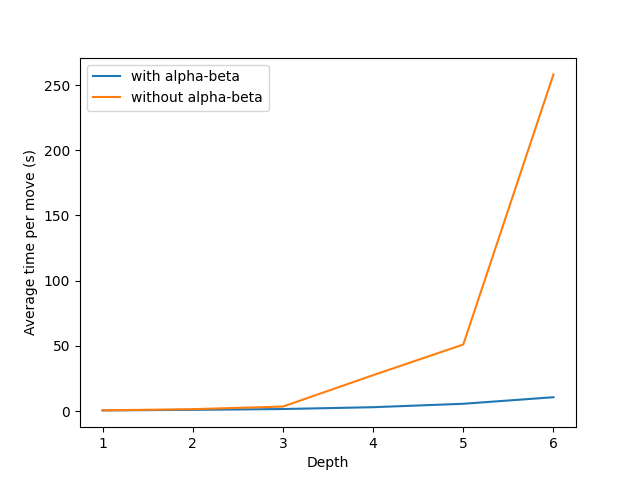
\includegraphics[width=0.8\textwidth]{../img/alpha-beta_comparison.png}
  \caption{Comparison of the average time taken to make a move by the minimax algorithm with and without alpha-beta pruning at various depths in the perfect information environment.}
  \label{WithWithoutAlphaBeta}
\end{figure}

\subsection{Alpha-Beta Pruning}

The minimax algorithm is capable of finding the optimal move in a two-player game by searching the entire game tree and considering all possible moves by both players. However, for some games, such as Durak, the game tree can be extremely large, making it computationally infeasible to fully explore. In these cases, the \textbf{alpha beta} pruning technique is used in conjunction with minimax to optimize the search process. Alpha beta pruning involves eliminating branches of the game tree that cannot affect the final decision, allowing the algorithm to focus its search on more promising areas of the tree and significantly reducing the overall computational burden \citep{AI4Ed}. Through comparison of the average time of the minimax algorithm with and without the implementation of alpha-beta pruning at various fixed depths in the perfect information environment, it is evident that the incorporation of alpha-beta pruning leads to a marked increase in efficiency (as depicted in Figure 3). At a depth of 6, the minimax algorithm incorporating alpha-beta pruning required an average of 10.6 milliseconds to explore the game tree, while the minimax without this optimization technique required an average of 258.2 milliseconds to do so. As anticipated, the use of alpha-beta pruning results in significantly faster performance compared to the minimax without this optimization technique.

\begin{figure}[h]
\captionsetup{justification=centering}
\begin{lstlisting}
function minimax(gameView, alpha, beta, depth, bestMove)
...
    bestVal = game.turn == 1 ? -infinity : +infinity
	
    possibleMoves = getPossibleMoves(gameView)
    for each move in possibleMoves
        gameViewCopy = copy(gameView)
        gameViewCopy.Move(move)
        v = minimax(gameViewCopy, alpha, beta, depth + 1, null)
        	
        if game.turn == 1 && v > bestVal or game.turn == 2 && v < bestVal then
            bestVal = v
            bestMove = move
        		
            if game.turn == 1 then 
                if v >= beta then 
                    return v
                alpha = Max(alpha, v)
            else
                if v <= alpha then
                    return v
                beta = Min(beta, v)
...
\end{lstlisting}
\caption{Part of the pseudocode of alpha-beta pruning technique inside the minimax \texttt{Move} method}
\label{fig:alphabeta}
\end{figure}

The implementation of this technique, given in Figure \ref{fig:alphabeta}, involves adding two additional parameters, ``alpha'' and ``beta'', to the minimax function. These parameters are initialized to negative and positive infinity, respectively, indicating that any minimax value is acceptable. The algorithm then compares the values of alpha and beta to the current minimax value during the search, and if the value exceeds a certain threshold, the search is terminated as a game-winning move has been identified. Overall, the incorporation of alpha-beta pruning into the minimax algorithm involves only a minor modification to the existing code, making it a useful tool for optimizing the performance of minimax in certain situations.

\subsection{State Caching}

Another method for optimizing the search of a game tree using the minimax algorithm was to implement state caching. This technique involves serializing the current game state with its current depth and storing its corresponding heuristic value in a cache. During the search process, the minimax agent can then check the cache before evaluating a given state. If the state has already been explored, the agent can retrieve the stored heuristic value and avoid the need to recalculate it, thereby reducing the overall computational complexity of the search. It was observed during the development of the program that the same game state may be encountered multiple times through different paths in the tree, making state caching an effective optimization technique for the minimax algorithm.

\begin{figure}[h]
  \centering
  \captionsetup{justification=centering}
  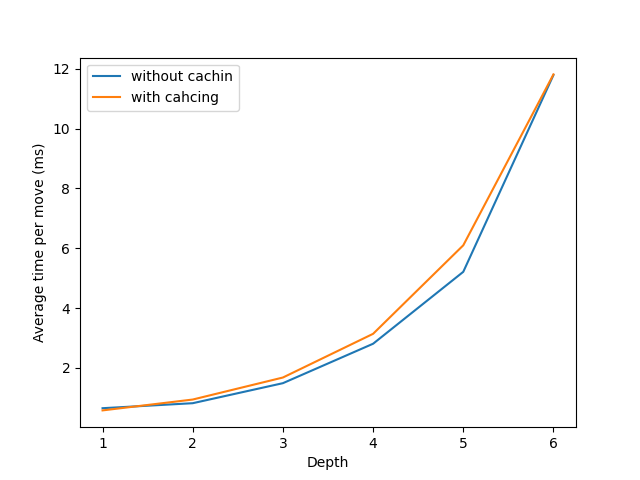
\includegraphics[width=0.8\textwidth]{../img/caching.png}
  \caption{Comparison of the average time taken to make a move by the minimax algorithm with and without cahcing of the states.}
  \label{WithWithoutAlphaBeta}
\end{figure}

The implementation of a caching system did not produce an improvement in the average time per move of the minimax algorithm. In fact, the results of the experiment demonstrated that in certain fixed depths, the use of caching resulted in slightly worse performance compared to not using caching. This unexpected outcome is illustrated in Figure 8 and warrants further investigation.

\section{Monte Carlo Tree Search Agent}
\label{MCTS}

Monte Carlo Tree Search (MCTS) is a search algorithm that is commonly used in games such as chess, Go, and other board games to find the best move to make. It is based on the idea of using random sampling to estimate the value of different moves, rather than explicitly searching through the entire game tree \citep{MCTSSurvey}.

The MCTS algorithm consists of four main steps at every iteration:

\begin{enumerate}
	\item Selection: The algorithm starts at the root of the game tree and selects successive child nodes by using a heuristic evaluation function to guide the search towards promising areas of the tree.
	
	\item Expansion: Once a leaf node (a node without any children) is reached, the algorithm creates one or more child nodes for that leaf node and performs a simulation from that point.
	
	\item Simulation: The simulation involves playing out a random sequence of moves from the current position to the end of the game, using a simple evaluation function to determine the outcome.
	
	\item Backpropagation: The results of the simulation are then propagated back up the tree, updating the values of the nodes visited during the selection and expansion steps.
	
\end{enumerate}

The MCTS algorithm repeats these steps until a sufficient number of iterations (in this program `limits') have been performed, at which point it selects the move with the highest estimated value as the best move to make. Considering the possibility of regrouping the four main steps in MCTS, this version of the algorithm works with two distinct policies: 

\begin{enumerate}
	\item Tree Policy: From the nodes contained within the search tree, either select a leaf node or create a new one by expanding the tree (selection and expansion).
	
	\item Default Policy: Evaluate a non-terminal state in the domain by simulating its progression to a terminal state and generating an estimate of its value (simulation).
\end{enumerate}

The backpropagation step does not involve the use of a policy itself, but rather adjusts the internal parameters of node statistics that inform future tree policy. These steps are summarized in the pseudocode in Figure \ref{fig:mctsGeneral}.


\begin{figure}[h]
\captionsetup{justification=centering}
\begin{lstlisting}
function MCTSSearch((*@$s_0$@*))
    create root node (*@$v_0$@*) from the tree with the state (*@$s_0$@*)
    while limit has not reached do
        (*@$v_l$@*) = TreePolicy((*@$v_0$@*))
        reward = DefaultPolicy(s((*@$v_l$@*))
        BackPropagation((*@$v_l$@*), reward)
    return a(BestChild((*@$v_0$@*), 0))
\end{lstlisting}
\caption{A general pseudocode for MCTS}
\label{fig:mctsGeneral}
\end{figure}

$v_0$ is the root node that corresponds to the state $s_0$. \texttt{TreePolicy} returns the last node, $v_l$, reached either by expanding or selecting the node, which corresponds to the state $s_l$. \texttt{DefaultPolicy} method simulates the whole game given the last node and returns the outcome of the playout from the state $s_l$, which is \texttt{result}. Given the \texttt{result} from the simulated game, the \texttt{BackPropagation} method adjusts the values from $v_l$ up until the root node $v_0$. Once the limit of computation is reached, the algorithm provides the result of the overall search \texttt{a(BestChild($v_0$))} where \texttt{a} is the action that provides the best move in the state $s_0$ of the root $v_0$.

The UCT (Upper Confidence bounds applied to Trees) algorithm is a heuristic method for finding the optimal move in a two-player game by considering both the exploration of new nodes in the search tree and the exploitation of known information about the value of certain nodes. It is a method that allows to find the best node in the \texttt{TreePolicy} method and best move given the root node \texttt{BestChild} method. It is commonly used in situations where it is necessary to balance the trade-off between exploration and exploitation in order to make the most informed decision. By using this approach, it is possible to effectively navigate the search tree and identify the best possible move, taking into account the inherent uncertainty and complexity of the game at hand \citep{MCTSSurvey}. To calculate the UCT value for each node, 

\[ UCT(v) = 1 - \frac{Q(v')}{N(v')} + c*\sqrt{\frac{2 * ln{N(v)}}{N(v')}} \]

is used. Every node has the value of \textit{Q(v)} that corresponds to the total reward of all playouts that passed through this state and the number \textit{N(v)} of times it has been visited. The \textit{c} value is the exploration constant that balances the exploration exploitation trade off. The reason why the 1 subtracts from fraction of \textit{Q(v)} and \textit{N(v)} is because we want to invert the win rate, i.e. the average reward, which will always be between 0 and 1. As an example, consider a scenario in a two-player game if a given move leads to an average reward of 0.3 for player 1, then the same move leads to an average reward of 0.7 for player 2. 

It is important to note that the calculation mentioned above assumes that moves strictly alternate between the two players, such that the first player makes a move, followed by the second player, and then the first player again, and so on. However, it is important to note that the alternating move structure mentioned previously does not always hold true in the game of Durak. Specifically, in Durak, the moves do not necessarily alternate between players. For example, if the first player makes an attack as their first move and the second player decides to take the cards, the first player may consecutively attack more until they no longer have the necessary card or simply choose not to attack any further. In this scenario, the move turn would not follow the alternating pattern described earlier. Because of that in cases where the moves do not strictly alternate between players, the win rate is not inverted as previously described. Instead, it is only inverted in cases where the turns alternate between players.

Now that we have a general understanding of MCTS and the Upper Confidence Bound applied to Trees (UCT) algorithms, it is time to explore the implementation of the TreePolicy, DefaultPolicy, and BackPropagation in these algorithms. The pseudocode of MCTS algorithm is depicted in Figure  \ref{fig:mctsREST}. 

For each node v, there are four pieces of data associated with it: the state s(v) corresponding to the node, the action a(v) that led to the node, the total simulation reward Q(v), and the number of visits N(v) to the node represented as a nonnegative integer. The term \texttt{reward} indicates the outcome of the simulated game and \texttt{f(s(v), a)} represents the function that takes state of the node and action as arguments and produces the new state. 

The return value of the overall search in this case is \texttt{a(BESTCHILD($v_0$, 0))} which will give the action \texttt{a} that leads to the child with the highest reward, since the exploration parameter \texttt{c} is set to 0 for this final call on the root node $v_0$. \citep{MCTSSurvey}.

It should be noted that the simulation process in the \texttt{DefaultPolicy} follows a random path through the search tree. While this approach allows for a broad exploration of potential moves, it may result in slower convergence and lower accuracy compared to using a more informed strategy for selecting simulation moves. In the program, it is possible to choose the simulation type when running experiments using MCTS. The options include using a random simulation (simulation=`random') or using a more informed strategy (simulation=`greedy'). The informed strategy employs a greedy agent to make decisions, which tends to guide the search more effectively towards areas of the tree that are more promising.

\begin{figure}[h]
\captionsetup{justification=centering}
\begin{lstlisting}
private void Backpropagation(Node nodeToExplore, int playoutResult)
{
    	while(tempNode != null)
    	{
		tempNode.IncrementPlayouts();
		// draw
		if (playoutResult == -1)
		{
			tempNode.AddScore(0.5);
		} 
		else if (tempNode.GetGame().Player() == playoutResult)
		{
			tempNode.AddScore(1.0);
		}
		tempNode = tempNode.GetParent();
	}
}
\end{lstlisting}
\caption{A snippet of Backpropagation method}
\label{fig:mctsBackpropagation}
\end{figure}

Upon receiving the reward result from the \texttt{DefaultPolicy}, the program passes this information to the \texttt{Backpropagation} function in order to update the values of the nodes in the path traversed during the simulation. These values include the visit count and the reward count, also known as the win count. In zero sum games, where one player's win corresponds to the other player's loss, the \texttt{Backpropagation} method increments the score of the winning player. However, in the card game Durak, there is the possibility of a draw between two players. To account for this possibility and ensure consistency in the scores, the \texttt{Backpropagation} method has been modified to include the case of a draw in its update process. The figure \ref{fig:mctsBackpropagation} illustrates the version of \texttt{Backpropagation} function that includes the case of draw. Specifically, the algorithm now awards a score of 0.5 to nodes in the case of a draw and a score of 1.0 in the case of a win.  


\begin{figure}[h]
\captionsetup{justification=centering}
\begin{lstlisting}
function MCTSSearch((*@$s_0$@*))
    create root node (*@$v_0$@*) from the tree with the state (*@$s_0$@*)
    while limit has not reached do
        (*@$v_l$@*) = TreePolicy((*@$v_0$@*))
        reward = DefaultPolicy(s((*@$v_l$@*))
        BackPropagation((*@$v_l$@*), reward)
    return a(BestChild((*@$v_0$@*), 0))
	
function TreePolicy(v)
    while v is nonterminal do 
        if v is not fully expanded then
            return Expand(v)
        else
            v = BestChild(v, c)
    return v

function Expand(v)
    get (*@ $a \in $ @*)first untried action from A(s(v))
    add a new child v' to v
        with s(v') = f(s(v), a) 
        and a(v') = a
    return v'
	
function BestChild(v, c)
    return (*@ $ \underset{v' \in children of v}{\arg\max} UCTValue(v,v',c) $ @*)
	
function UCTValue(v,v',c)
    avgReturn = (*@ $ \frac{Q(v')}{N(v')} $ @*)
    if Turn(v) != Turn(v') then 
        avgReturn = 1 - avgReturn
    return (*@ $ avgReturn + c * \sqrt{\frac{2 * ln{N(v)}}{N(v')}} $ @*)
	
function DefaultPolicy(s)
    while s is non-terminal do
        choose (*@ $a \in $ @*) A(s) uniformly at random
        s = f(s,a)
    return reward for state s

function Backpropagation(s, reward)
    while v is not null do
        N(v) = N(v) + 1
        Q(v) = Q(v) + reward
        v = parent of v
\end{lstlisting}
\caption{A MCTS Pseudocode}
\label{fig:mctsREST}
\end{figure}

\section{Closed World Sampling}
\label{closedWorld}
It is well-known that algorithms such as Minimax and Monte Carlo Tree Search (MCTS) can provide optimal play in games by thoroughly exploring the game tree. However, in imperfect information games such as Durak, this is not considered fair play because it allows the agent to access hidden information that it would not normally have access to. One way this can be done is through the use of a cloning method, which allows the agent to create a copy of the current game state and explore the potential outcomes of different moves. While this is acceptable in games with perfect information, such as chess or checkers, it is considered cheating in games with hidden information.

One way to address the issue of hidden information in imperfect information games is to use a \textbf{sampling} method that randomly generates a game state based on the information that the player can currently observe. This allows the agent to explore and evaluate potential moves without access to hidden information. The agent can then repeat this process a number of times, using algorithms such as Minimax or MCTS to determine the best course of action in each sampled game state. By considering the outcomes of these randomized scenarios, the agent can make a decision that is likely to be successful across a range of potential game states. This approach is called  ``Perfect Information Monte Carlo'' \citep{PerfectInformationMC}.

To implement a closed world sampling method in the game of Durak, a shuffled copy, \texttt{ShuffleCopy}, method was developed. In this game, the hidden information in the early stages of play includes the cards in the deck and the opponent's hand. To generate a randomly shuffled game state, the \texttt{ShuffleCopy} method combines these two sources of hidden information and shuffles them, before redistributing the same number of cards to the player and the deck. This process is represented in the Figure \ref{fig:shuffleCopy}. This shuffled game state is then returned to the calling agent, which can be either a Minimax or a MCTS. Thanks to that the shuffling process preserves the hidden information while allowing the agent to determine the best move to make in the current game state.

\begin{figure}[h]
\captionsetup{justification=centering}
\begin{lstlisting}
public Durak ShuffleCopy()
{
	// perform copy
    	Durak copy = (Durak)this.MemberwiseClone();
	...
	
    	Player opponent = copy.players[GetNextTurn()];
    	var opponentHiddenCards = opponent.GetHand().Where(c => !c.GetSeen());
    	int totalHiddenCards = opponentHiddenCards.Count();

    	// add hidden cards from opponent's hand to the hidden deck cards
    	copy.deck.GetCards().AddRange(opponentHiddenCards);
    	// remove hidden cards from the hand
    	opponent.GetHand().RemoveAll(card => !card.GetSeen());

    	// shuffle the unseen cards 
    	copy.deck.Shuffle();
	...
	
    	return copy;
}
\end{lstlisting}
\caption{A snipped of code that demonstrate the shuffling of the cards from the deck and opponent's hand inside the ShuffleCopy method}
\label{fig:shuffleCopy}
\end{figure}

The number of samples to be generated by the agents is determined by the user. A larger number of samples can lead to a more accurate result, but it also increases the time required to find the best move. To determine the optimal move after a certain number (n) of samples have been generated, the agents can keep track of the best moves identified in each shuffled game state. As the agents, such as Minimax and MCTS, evaluate each shuffled game state, they can store the results in a cache that tracks the frequency of each move. Once all n samples have been played, the agent can select the move that was identified as the best option in the greatest number of these scenarios.

\subsection{Parameter Specification}
\label{paramSpecification}

\subsubsection{Minimax}

In order to conduct an experiment using the minimax agent, it is necessary to specify certain parameters, which have been informed by our understanding of the minimax agent. Specifically, it is necessary to specify the value of the \texttt{depth} parameter, which determines the depth to which the search tree will be explored in order to identify the optimal move. In addition to the depth parameter, it is also necessary to specify the \texttt{eval} parameter, which specifies the heuristic function used to evaluate the state when the maximum depth has been reached. The \texttt{eval} parameter can take on either the value \texttt{basic} or \texttt{playout}. It is worth noting that, in a closed world scenario, the \texttt{samples} parameter is optional and has a default value of 20. The \texttt{samples} parameter serves to prevent agents such as Minimax and MCTS from cheating by accessing information about future states of the game (details in Section \ref{closedWorld}). This illustration presents an example of a simulation between the Minimax and greedy agents with arbitrary parameter values in the open and closed world:\\

\textbf{Open-world: }
\begin{lstlisting}
dotnet run -ai1=minimax:depth=4,eval=basic -ai2=greedy -open_world
\end{lstlisting}

\textbf{Closed-world: }
\begin{lstlisting}
dotnet run -ai1=minimax:depth=6,eval=basic,samples=15 -ai2=smart
\end{lstlisting}

\subsubsection{MCTS}

Regarding MCTS,it is necessary to specify the value of the \texttt{limit} parameter, which determines the computational budget allocated for the algorithm to build the search tree. The search is halted and the best-performing root action is returned once this budget is reached. The \texttt{c}, which is called exploration constant, parameter also needs to be specified because it determines the balance between exploitation and exploration in the UCB equation. This parameter is set to a default value of  $\sqrt{2}$ ($\approx 1.41$) and can be adjusted to fine-tune the performance of the algorithm. The \texttt{simulation} parameter should also be specified, indicating whether to use a smart simulation (\texttt{greedy}) or a random simulation (\texttt{random}). Lastly, in a closed world setting, just like in Minimax, it is necessary to specify the \texttt{samples} parameter to prevent the MCTS agent from cheating by considering future states of the game. This example demonstrates a simulation between MCTS and greedy agents with arbitrary parameter values in open and closed world settings: \\

\textbf{Open-world: }
\begin{lstlisting}
dotnet run -ai1=mcts:limit=100,simulation=greedy -ai2=greedy 
							-open_world
\end{lstlisting}

\textbf{Closed-world: }
\begin{lstlisting}
dotnet run -ai1=mcts:limit=100,simulation=greedy,samples=10 
							-ai2=greedy
\end{lstlisting}





